\chapter{Opracowanie wyników}

Rozdział ten zawiera analizę wyników działania programu opisanego w~części~\ref{cha:implementacja}. Przeprowadzono także weryfikację wpływu usunięcia pojedynczego posterunku opadowego na uzyskane wskazanie opadowe na obszarze, co było jednym z~celów tej pracy.


\section{Wielkość błędu}
asdasd

\section{Warianty opadu}
Opisany w~rozdziale~\ref{cha:implementacja} program został uruchomiony celem wyznaczenia wartości opadu powierzchniowego dla obu przygotowanych wariantów funkcji opadowej. Poniżej zaprezentowano uzyskane wyniki.

\begin{table}[!ht]
\caption{Wyniki działania programu}
\begin{center}
\begin{tabular}{|c|c|c|c|}
\hline
 Wariant      & Opad wyznaczony [$m^3$] & Opad rzeczywisty [$m^3$] & Różnica [\%] \\ \hline \hline

 Paraboliczny & 1 462 995 563.4253  &   1 500 568 329.7155  &  -2.5039 \\ \hline
 Wymierny     & 1 559 081 843.8972  &   1 571 689 381.8665  &  -0.8022 \\ \hline

\end{tabular}
\end{center}
\end{table}

Jak można zauważyć, dla wariantu z~opadem parabolicznym mamy do czynienia z~niedomiarem. Jest to spodziewana sytuacja wynikająca z~interpolowania funkcji wklęsłej. Różnica z~rzeczywistą objętością opadu wynosi ok. 2.5 \%, zatem jest to zadowalający wynik.

W przypadku wymiernego opadu uzyskano jeszcze lepsze wyniki. Błąd wyznaczonej wartości jest mniejszy niż jeden procent, a~należy zwrócić uwagę, dane przygotowane na potrzeby testów obejmują obszar rzędu stu tysięcy kilometrów kwadratowych.



\section{Analiza wrażliwości na posterunki opadowe}
W~tej części przeprowadzono wpływ wyłączenia wskazanego posterunku opadowego (ograniczono się do wybory punktów zawartych w granicach wskazanej zlewni) na wynik działania omawianej metody. Pozwala to znaleźć odpowiedź na pytanie: \textit{Czy sieć istniejących posterunków opadowych jest wystarczająca?}, a~to pomoże podejmować decyzje o~zwiększaniu ilości owych posterunków bądź przeniesieniu w~inną lokalizację.

Rysunek~\ref{fig:identyfikatory} przedstawia identyfikatory wykluczanych z~analizy punktów, natomiast wiersze tabeli prezentują rezultat działania programu bez zadanego punktu.

\begin{figure}[!ht]
	\centering
	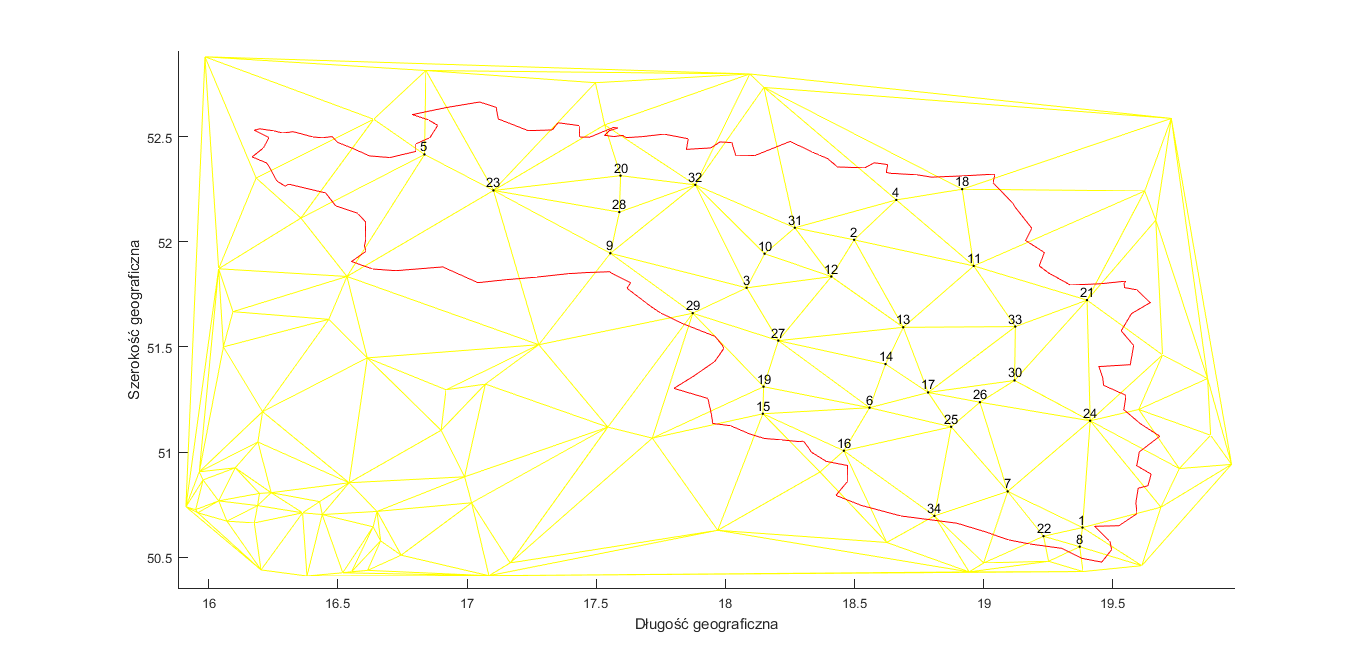
\includegraphics[width=1\linewidth]{identyfikatory_punktow}
	\label{fig:identyfikatory}
	\caption{Identyfikatory posterunków wewnątrz zlewni}
\end{figure}

\subsection{Opad paraboliczny}

\begin{table}[!ht]
\label{tab:wyniki_wymierna}
\caption{Wpływ usunięcia posterunku na wynik algorytmu. Wariant paraboliczny.}
\begin{center}
\begin{tabular}{|c|l|l|r@{.}l|r@{.}l|r@{.}l|}
%nagłówek tabeli
\cline{2-3} \cline{6-9}
\multicolumn{1}{l}{} & \multicolumn{2}{|c|}{Opad $[m^3]$} & \multicolumn{2}{c}{} & \multicolumn{4}{|c|}{Wpływ posterunku} \\
\hline Posterunek & Wyznaczony & Rzeczywisty & \multicolumn{2}{c}{Różnica [\%]} & \multicolumn{2}{|c|}{[$m^3$]}& \multicolumn{2}{|c|}{$\times 10^{-3} [\%]$} \\ \hline \hline

--    &     1462995563.42529   &    1500568329.7155    &      -2 & 5039  &              0 & 00          &     0 & 00 \\ \hline
1   &     1463076745.52465   &    1500568302.6776    &      -2 & 4984  &          81182 & 0994   &     5 & 55 \\ \hline
2   &     1461776787.89791   &    1500568329.7155    &      -2 & 5851  &       -1218775 & 5274   &   -83 & 31 \\ \hline
3   &     1462473733.66747   &    1500568329.7155    &      -2 & 5386  &        -521829 & 7578   &   -35 & 67 \\ \hline
4   &     1460378875.61033   &    1500568329.7155    &      -2 & 6782  &       -2616687 & 8150   &  -178 & 86 \\ \hline
5   &     1468988504.71699   &    1500568343.3016    &      -2 & 1045  &        5992941 & 2917   &   409 & 64 \\ \hline
6   &     1461622417.1231    &    1500568329.7155    &      -2 & 5954  &       -1373146 & 3022   &   -93 & 86 \\ \hline
7   &     1464682183.90386   &    1500568361.4533    &      -2 & 3915  &        1686620 & 4786   &   115 & 29 \\ \hline
8   &     1462995563.42529   &    1500568329.7155    &      -2 & 5039  &             -0 & 0000   &     0 & 00 \\ \hline
9   &     1453656531.65409   &    1500568329.7155    &      -3 & 1262  &       -9339031 & 7712   &  -638 & 35 \\ \hline
10  &     1462338580.82334   &    1500568329.7155    &      -2 & 5476  &        -656982 & 6020   &   -44 & 91 \\ \hline
11  &     1454316634.11975   &    1500568329.7155    &      -3 & 0822  &       -8678929 & 3055   &  -593 & 23 \\ \hline
12  &     1460880307.4094    &    1500568329.7155    &      -2 & 6448  &       -2115256 & 0159   &  -144 & 58 \\ \hline
13  &     1460206170.95541   &    1500568329.7155    &      -2 & 6897  &       -2789392 & 4699   &  -190 & 66 \\ \hline
14  &     1461450430.25043   &    1500568329.7155    &      -2 & 6068  &       -1545133 & 1749   &  -105 & 61 \\ \hline
15  &     1462002685.70473   &    1500568329.7155    &      -2 & 5700  &        -992877 & 7206   &   -67 & 87 \\ \hline
16  &     1462214551.12403   &    1500568329.7155    &      -2 & 5559  &        -781012 & 3013   &   -53 & 38 \\ \hline
17  &     1462691315.16175   &    1500568329.7155    &      -2 & 5241  &        -304248 & 2635   &   -20 & 80 \\ \hline
18  &     1464582760.98511   &    1500568329.7155    &      -2 & 3981  &        1587197 & 5598   &   108 & 49 \\ \hline
19  &     1461064560.9566    &    1500568329.7155    &      -2 & 6325  &       -1931002 & 4687   &  -131 & 99 \\ \hline
20  &     1461310691.73423   &    1500568329.7155    &      -2 & 6161  &       -1684871 & 6911   &  -115 & 17 \\ \hline
21  &     1459561769.38071   &    1500568329.7155    &      -2 & 7327  &       -3433794 & 0446   &    -0 & 23 \\ \hline
22  &     1463418751.62474   &    1500568331.6960    &      -2 & 4757  &         423188 & 1994   &    -0 & 03 \\ \hline
23  &     1453767799.36506   &    1500568329.7155    &      -3 & 1189  &       -9227764 & 0602   &    -0 & 63 \\ \hline
24  &     1462113590.39904   &    1500568331.1793    &      -2 & 5627  &        -881973 & 0263   &    -0 & 06 \\ \hline
25  &     1461120846.70184   &    1500568329.7155    &      -2 & 6288  &       -1874716 & 7235   &    -0 & 13 \\ \hline
26  &     1462704787.16475   &    1500568329.7155    &      -2 & 5233  &        -290776 & 2605   &    -0 & 02 \\ \hline
27  &     1460220263.75282   &    1500568329.7155    &      -2 & 6889  &       -2775299 & 6725   &    -0 & 19 \\ \hline
28  &     1461578202.47148   &    1500568329.7155    &      -2 & 5984  &       -1417360 & 9538   &    -0 & 10 \\ \hline
29  &     1461321743.5352    &    1500568329.7155    &      -2 & 6154  &       -1673819 & 8901   &    -0 & 11 \\ \hline
30  &     1460813336.266     &    1500568329.7155    &      -2 & 6493  &       -2182227 & 1593   &    -0 & 15 \\ \hline
31  &     1460877238.93555   &    1500568329.7155    &      -2 & 6451  &       -2118324 & 4897   &    -0 & 14 \\ \hline
32  &     1461214840.52951   &    1500568329.7155    &      -2 & 6226  &       -1780722 & 8958   &    -0 & 12 \\ \hline
33  &     1460597607.61728   &    1500568329.7155    &      -2 & 6637  &       -2397955 & 8080   &    -0 & 16 \\ \hline
34  &     1462056933.32981   &    1500568329.7155    &      -2 & 5665  &        -938630 & 0955   &    -0 & 06 \\ \hline



\end{tabular}
\end{center}
\end{table}


\subsection{Opad wymierny}

